% =============================================================================
%  Neural Network Track Extrapolation for the LHCb Upgrade II
%  Author: G. Scriven (LHCb, Nikhef)
%  Date:   March 2026
% =============================================================================
\documentclass[aspectratio=169, 11pt]{beamer}

% ---- Theme & Colours --------------------------------------------------------
\usetheme{Madrid}
\usecolortheme{default}

\definecolor{lhcbblue}{HTML}{1F77B4}
\definecolor{nngreen}{HTML}{2CA02C}
\definecolor{rkorange}{HTML}{FF7F0E}
\definecolor{rk4red}{HTML}{D62728}
\definecolor{lightgray}{HTML}{F0F0F0}
\definecolor{darkgray}{HTML}{404040}
\definecolor{cachegreen}{HTML}{27AE60}
\definecolor{cachered}{HTML}{E74C3C}

\setbeamercolor{title}{fg=white, bg=lhcbblue}
\setbeamercolor{frametitle}{fg=white, bg=lhcbblue}
\setbeamercolor{structure}{fg=lhcbblue}
\setbeamercolor{block title}{bg=lhcbblue!20, fg=black}
\setbeamercolor{block body}{bg=lhcbblue!5}
\setbeamercolor{block title alerted}{bg=rk4red!20, fg=black}
\setbeamercolor{block body alerted}{bg=rk4red!5}
\setbeamercolor{block title example}{bg=nngreen!20, fg=black}
\setbeamercolor{block body example}{bg=nngreen!5}
\setbeamertemplate{navigation symbols}{}
\setbeamertemplate{footline}[frame number]

% ---- Packages ---------------------------------------------------------------
\usepackage[utf8]{inputenc}
\usepackage[T1]{fontenc}
\usepackage{lmodern}
\usepackage{amsmath,amssymb,mathtools}
\usepackage{booktabs}
\usepackage{array}
\usepackage{colortbl}
\usepackage{graphicx}
\usepackage{xcolor}
\usepackage{tikz}
\usetikzlibrary{arrows.meta, positioning, shapes.geometric, calc,
                decorations.pathreplacing, fit}
\usepackage{listings}
\usepackage{multicol}
\usepackage{hyperref}
\usepackage{caption}

% ---- Listings style for pseudo-code ----------------------------------------
\lstset{
  basicstyle=\ttfamily\scriptsize,
  keywordstyle=\color{lhcbblue}\bfseries,
  commentstyle=\color{gray}\itshape,
  stringstyle=\color{nngreen},
  columns=fullflexible,
  keepspaces=true,
  frame=single,
  backgroundcolor=\color{lightgray},
  breaklines=true,
  tabsize=2,
  morekeywords={for, if, return, void, float, int, const, auto},
}

% ---- Custom commands --------------------------------------------------------
\newcommand{\dz}{\Delta z}
\newcommand{\qop}{q/p}
\newcommand{\bvec}[1]{\mathbf{#1}}
\newcommand{\vstate}{\bvec{s}}
\newcommand{\clgt}{c_\text{light}}
\newcommand{\tx}{t_x}
\newcommand{\ty}{t_y}
\newcommand{\zfrac}{\zeta}

% Graphics path
\graphicspath{
  {experiments/field_maps/field_nn/}
  {experiments/field_maps/field_nn/analysis/}
  {experiments/field_maps/field_nn/doc/plots/}
  {experiments/gen_1/}
  {experiments/gen_1/V3/analysis/}
  {legacy/plots/}
}

% =============================================================================
\title[NN Track Extrapolation]{%
  \textbf{Neural Network Track Extrapolation}\\[4pt]
  \large for the LHCb Upgrade~II}

\author{G.~Scriven}
\institute{LHCb\quad$\cdot$\quad Nikhef}
\date{March 2026}

\begin{document}

% =============================================================================
% TITLE SLIDE
% =============================================================================
\begin{frame}[plain]
  \titlepage
\end{frame}

% =============================================================================
% OUTLINE
% =============================================================================
\begin{frame}{Outline}
  \tableofcontents
\end{frame}


% #############################################################################
\section{Motivation}
% #############################################################################

% =============================================================================
\begin{frame}{Why Now? --- The LHCb Upgrade~II Challenge}

\begin{columns}[T]
\begin{column}{0.55\textwidth}
  \begin{itemize}
    \item LHCb Upgrade~II: instantaneous luminosity increases to
          $\mathcal{L} = 1.5\times10^{34}~\text{cm}^{-2}\text{s}^{-1}$
    \item $\sim$5--10$\times$ more tracks per event
    \item Track extrapolation = propagating charged particles through
          the dipole magnet via Runge--Kutta integration
    \item \textbf{Current cost}: $\sim$8.35~$\mu$s/track
    \item Magnetic field lookups dominate: \alert{76\%} of total time
    \item[$\Rightarrow$] Two strategies to accelerate:
  \end{itemize}

  \vspace{6pt}
  \begin{enumerate}
    \item \textcolor{nngreen}{\textbf{NN field surrogate}}: replace field
          lookup with a cache-friendly neural network
    \item \textcolor{lhcbblue}{\textbf{NN full extrapolation}}: replace
          the entire RK integration with a single forward pass
  \end{enumerate}
\end{column}

\begin{column}{0.43\textwidth}
  \begin{figure}
    
\includegraphics[width=\textwidth]{stacked_and_amdahl.pdf}
    \caption*{\scriptsize RK sub-operation cost breakdown and\\Amdahl's Law
              projection for field acceleration}
  \end{figure}
\end{column}
\end{columns}
\end{frame}


% #############################################################################
\section{Track Extrapolation \& Runge--Kutta Schemes}
% #############################################################################

% =============================================================================
\begin{frame}{The Track State Vector}

All LHCb extrapolators represent the track state at position~$z$ as:
\begin{equation*}
  \vstate = \begin{pmatrix} x \\ y \\ \tx \\ \ty \\ \qop \end{pmatrix}
  \quad\text{at position } z
\end{equation*}

\begin{itemize}
  \item $x, y$: transverse positions (mm)
  \item $\tx = dx/dz$, $\ty = dy/dz$: direction tangents (slopes)
  \item $\qop$: charge / total momentum ($\text{MeV}^{-1}$)
  \item Independent variable is $z$ (beam axis), not time
\end{itemize}

\vspace{6pt}
\textbf{Covariance propagation} via the $5\times5$ transport matrix~$F$:
\begin{equation*}
  C_\text{out} = F \, C_\text{in} \, F^T
\end{equation*}
\end{frame}


% =============================================================================
\begin{frame}{Equations of Motion --- Lorentz Force}

A charged particle in field $\bvec{B} = (B_x, B_y, B_z)$ obeys:
\begin{equation*}
  \frac{d}{dz}
  \begin{pmatrix} x \\ y \\ \tx \\ \ty \end{pmatrix}
  =
  \begin{pmatrix} \tx \\ \ty \\
    (\qop)\,\clgt\, \mathcal{A}_x \\
    (\qop)\,\clgt\, \mathcal{A}_y
  \end{pmatrix}
\end{equation*}

where $n = \sqrt{1 + \tx^2 + \ty^2}$ (arc-length correction) and:

\begin{align*}
  \mathcal{A}_x &= n\bigl[\,\ty(\tx B_x + B_z) - (1+\tx^2)\,B_y\,\bigr]
  \\[4pt]
  \mathcal{A}_y &= n\bigl[\,-\tx(\ty B_y + B_z) + (1+\ty^2)\,B_x\,\bigr]
\end{align*}

\vspace{4pt}
\begin{block}{Physical interpretation}
  \begin{itemize}
    \item Positions evolve linearly through slopes
    \item Slopes change due to the magnetic field --- this is the bending
    \item Coupling $\kappa = (\qop)\,\clgt \propto q/p$: low-momentum
          particles bend more
  \end{itemize}
\end{block}
\end{frame}


% =============================================================================
\begin{frame}{The LHCb Dipole Field}

\begin{columns}[T]
\begin{column}{0.48\textwidth}
  The vertical field $B_y$ is \emph{not} uniform --- it varies by a
  factor of ${\sim}3\times$ across the magnet:

  \vspace{6pt}
  \begin{table}
  \centering\small
  \begin{tabular}{@{} r r c @{}}
    \toprule
    $z$ (mm) & $B_y$ (T) & Rel.\ curvature \\
    \midrule
    0    & 1.10 & $1.65\times$ \\
    2000 & 0.95 & $1.43\times$ \\
    4000 & 0.70 & $1.05\times$ \\
    6000 & 0.50 & $0.75\times$ \\
    8000 & 0.40 & $0.60\times$ \\
    \bottomrule
  \end{tabular}
  \end{table}

  \vspace{6pt}
  \begin{alertblock}{Key constraint}
    Any model that cannot represent \textbf{position-dependent curvature}
    will inevitably fail.
  \end{alertblock}
\end{column}

\begin{column}{0.50\textwidth}
  \begin{figure}
    
\includegraphics[width=\textwidth]{field_cost_vs_momentum.pdf}
    \caption*{\scriptsize Field evaluation cost varies with track
              momentum --- low-$p$ tracks require more RK steps.}
  \end{figure}
\end{column}
\end{columns}
\end{frame}


% =============================================================================
\begin{frame}{Embedded Runge--Kutta Framework}

An embedded RK method of order $p(p{-}1)$ computes \textbf{two estimates}
per step, defined by its \textbf{Butcher tableau}:

\begin{equation*}
  \renewcommand{\arraystretch}{1.2}
  \begin{array}{c|cccc}
    c_1    & & & & \\
    c_2    & a_{21} & & & \\
    \vdots & \vdots & \ddots & & \\
    c_s    & a_{s1} & \cdots & a_{s,s-1} & \\
    \hline
           & b_1 & b_2 & \cdots & b_s \\
           & b^*_1 & b^*_2 & \cdots & b^*_s
  \end{array}
\end{equation*}

\begin{align*}
  \text{Stages:}\quad & \bvec{k}_i = h\,\bvec{f}\!\left(z_n + c_i h,\;
    \bvec{y}_n + \textstyle\sum_{j<i} a_{ij}\,\bvec{k}_j\right) \\[4pt]
  \text{Update:}\quad & \bvec{y}_{n+1} = \bvec{y}_n +
    \textstyle\sum_{i} b_i\,\bvec{k}_i \quad\text{(order $p$)} \\[4pt]
  \text{Error:}\quad  & \bvec{e} = \textstyle\sum_{i}(b_i - b^*_i)\,\bvec{k}_i
\end{align*}
\end{frame}


% =============================================================================
\begin{frame}{Cash--Karp 5(4) --- The LHCb Default}

\textbf{6 stages}, 5th-order with 4th-order error estimate:

\begin{equation*}
\renewcommand{\arraystretch}{1.1}
{\footnotesize
\begin{array}{c|cccccc}
  0          &   \\
  \frac{1}{5}      & \frac{1}{5} \\
  \frac{3}{10}     & \frac{3}{40}    & \frac{9}{40} \\
  \frac{3}{5}      & \frac{3}{10}    & -\frac{9}{10}  & \frac{6}{5} \\
  1          & -\frac{11}{54}& \frac{5}{2}    & -\frac{70}{27}& \frac{35}{27} \\
  \frac{7}{8}      & \frac{1631}{55296} & \frac{175}{512} &
    \frac{575}{13824} & \frac{44275}{110592} & \frac{253}{4096} \\[4pt]
  \hline
  b_i  & \frac{37}{378} & 0 & \frac{250}{621} & \frac{125}{594} & 0 &
    \frac{512}{1771} \\[3pt]
  b^*_i & \frac{2825}{27648} & 0 & \frac{18575}{48384} &
    \frac{13525}{55296} & \frac{277}{14336} & \frac{1}{4}
\end{array}
}
\end{equation*}

\vspace{4pt}
\begin{itemize}
  \item Minimises leading truncation error of 5th-order formula
  \item $c_6 = 7/8$ (interior) gives more reliable step-size estimates
  \item Preferred over Fehlberg for non-stiff systems like tracking
\end{itemize}
\end{frame}


% =============================================================================
\begin{frame}{The RK Scheme Zoo --- 15 Methods Available}

\begin{table}
\centering\small
\begin{tabular}{@{}lcccl@{}}
  \toprule
  \textbf{Scheme} & \textbf{Stages} & \textbf{Order} & \textbf{FSAL} &
    \textbf{Cost (field evals)} \\
  \midrule
  Cash--Karp (default) & 6 & 5(4) & No & 6/step \\
  Dormand--Prince      & 7 & 5(4) & Yes & 6/step (FSAL) \\
  Bogacki--Shampine~3  & 4 & 3(2) & No & 4/step \\
  Bogacki--Shampine~5  & 8 & 5(4) & No & 8/step \\
  Heun--Euler          & 2 & 2(1) & No & 2/step \\
  Tsitouras~5          & 7 & 5(4) & Yes & 6/step (FSAL) \\
  Sharp--Verner~6      & 9 & 6(5) & Yes & 8/step (FSAL) \\
  Sharp--Verner~7      & 12& 7(6) & Yes & 11/step (FSAL) \\
  Verner~6             & 8 & 6(5) & No & 8/step \\
  Verner~7             & 10& 7(6) & No & 10/step \\
  Verner~8             & 13& 8(7) & No & 13/step \\
  Verner~9             & 16& 9(8) & No & 16/step \\
  \bottomrule
\end{tabular}
\end{table}

\vspace{4pt}
\begin{itemize}
  \item FSAL = First Same As Last: last stage of step $n$ = first of $n{+}1$
  \item Higher-order methods take \textbf{larger steps} for the same tolerance
        $\Rightarrow$ fewer total field evaluations
\end{itemize}
\end{frame}


% =============================================================================
\begin{frame}{Adaptive Step-Size Control}

The step is accepted/rejected based on the normalised error:
\begin{equation*}
  E = \max\!\left(
    \frac{|e_x|}{\epsilon_x},\;
    \frac{|e_y|}{\epsilon_y},\;
    \frac{|e_{\tx}|}{\epsilon_{\tx} + |\Delta\tx|\,\epsilon_\text{rel}}
  \right)
\end{equation*}

\begin{itemize}
  \item \textbf{Accept} if $E \leq \sigma$ (default $\sigma=5.5$)
  \item Mixed absolute--relative criterion for slopes prevents overly small
        steps in high-curvature regions
\end{itemize}

\vspace{4pt}
\textbf{PI controller} for step scaling:
\begin{equation*}
  h_{n+1} = h_n \cdot \text{clamp}\!\left(f,\; 0.125,\; 4.0\right),
  \quad
  f = \begin{cases}
    E^{-1/4}  & \text{shrink (order $p{-}1$)} \\
    E^{-1/5}  & \text{grow (order $p$)}
  \end{cases}
\end{equation*}

\vspace{4pt}
\textbf{Termination}: curling ($|\tx|,|\ty|>10$), excessive curvature
($|(\qop)B_y|>1/\text{m}$), step count $\geq 1000$, or out-of-bounds.
\end{frame}


% =============================================================================
\begin{frame}{Jacobian Propagation --- Variational Equations}

The $5\times5$ transport matrix has the structure ($\qop$ constant in RK step):
\begin{equation*}
  F =
  {\small\begin{pmatrix}
    1 & 0 & J_{x,\tx}   & J_{x,\ty}   & J_{x,\qop}\clgt \\
    0 & 1 & J_{y,\tx}   & J_{y,\ty}   & J_{y,\qop}\clgt \\
    0 & 0 & J_{\tx,\tx} & J_{\tx,\ty} & J_{\tx,\qop}\clgt \\
    0 & 0 & J_{\ty,\tx} & J_{\ty,\ty} & J_{\ty,\qop}\clgt \\
    0 & 0 & 0            & 0            & 1
  \end{pmatrix}}
\end{equation*}

The slope Jacobian evolves as:
\begin{equation*}
  \frac{d}{dz}\!\begin{pmatrix} J_{\tx} \\ J_{\ty} \end{pmatrix}
  = \frac{q}{p}\clgt
  \begin{pmatrix}
    \partial_{\tx}\mathcal{A}_x & \partial_{\ty}\mathcal{A}_x \\
    \partial_{\tx}\mathcal{A}_y & \partial_{\ty}\mathcal{A}_y
  \end{pmatrix}
  \!\begin{pmatrix} J_{\tx} \\ J_{\ty} \end{pmatrix}
\end{equation*}

with position Jacobians obtained by integration: $J_x = \int J_{\tx}\,dz$.
Solved simultaneously alongside the trajectory using the \textbf{same} RK
stages.
\end{frame}


% =============================================================================
\begin{frame}{Master Extrapolator --- Production Dispatch}

\begin{columns}[T]
\begin{column}{0.48\textwidth}
  \vspace{-6pt}
  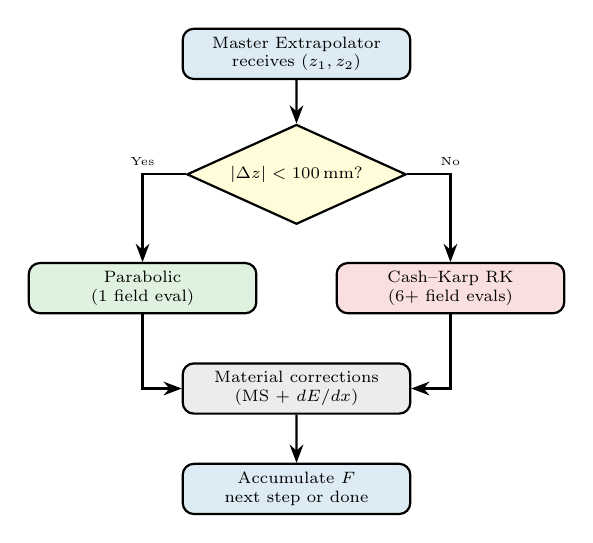
\begin{tikzpicture}[
    box/.style={draw, rounded corners, minimum width=3.4cm,
                minimum height=0.75cm, align=center, font=\scriptsize},
    decision/.style={draw, diamond, aspect=2.2, minimum width=2cm,
                     align=center, font=\scriptsize},
    >=Stealth, thick, scale=0.85, every node/.style={scale=0.85}
  ]
    \node[box, fill=lhcbblue!15] (master) at (0,0)
      {Master Extrapolator\\receives $(z_1, z_2)$};
    \node[decision, fill=yellow!15] (check) at (0,-1.8)
      {$|\dz| < 100$\,mm?};
    \node[box, fill=nngreen!15] (parab) at (-2.3,-3.5)
      {Parabolic\\(1 field eval)};
    \node[box, fill=rk4red!15] (rk) at (2.3,-3.5)
      {Cash--Karp RK\\(6+ field evals)};
    \node[box, fill=gray!15] (mat) at (0,-5.0)
      {Material corrections\\(MS + $dE/dx$)};
    \node[box, fill=lhcbblue!15] (accum) at (0,-6.5)
      {Accumulate $F$\\next step or done};

    \draw[->] (master) -- (check);
    \draw[->] (check) -| node[above,font=\tiny]{Yes} (parab);
    \draw[->] (check) -| node[above,font=\tiny]{No} (rk);
    \draw[->] (parab) |- (mat);
    \draw[->] (rk) |- (mat);
    \draw[->] (mat) -- (accum);
  \end{tikzpicture}
\end{column}

\begin{column}{0.50\textwidth}
  \textbf{Stepping \& material corrections:}
  \begin{enumerate}\small
    \item Divide total $\dz$ into steps $\leq 1000$~mm
    \item For each step:
    \begin{itemize}\scriptsize
      \item Validate: $|x|,|y|<10$~m, $|\tx|,|\ty|<5$
      \item Select sub-extrapolator
      \item Propagate state
      \item Accumulate: $F_\text{tot} = F_\text{step}\cdot F_\text{prev}$
    \end{itemize}
    \item If enabled, apply:
    \begin{itemize}\scriptsize
      \item \textbf{Multiple scattering} (angular broadening)
      \item \textbf{Energy loss} ($dE/dx$)
      \item \textbf{Electron bremsstrahlung}
    \end{itemize}
  \end{enumerate}

  \vspace{6pt}
  \begin{block}{100\,mm threshold}
    Parabolic: $\mathcal{O}(\dz^3)$ error, 1 field eval.\\
    For $|\dz|<100$~mm: error $\lesssim 10^{-4}$~mm.
  \end{block}
\end{column}
\end{columns}
\end{frame}


% =============================================================================
\begin{frame}{Profiling: Where the Time Goes}

\begin{columns}[T]
\begin{column}{0.48\textwidth}
  \begin{figure}
    
\includegraphics[width=\textwidth]{sub_operation_breakdown.pdf}
    \caption*{\scriptsize RDTSC cycle-level cost breakdown per RK step.}
  \end{figure}
\end{column}

\begin{column}{0.48\textwidth}
  \begin{figure}
    
\includegraphics[width=\textwidth]{field_call_speed_and_amdahl.pdf}
    \caption*{\scriptsize Field call cost \& Amdahl's law analysis.}
  \end{figure}
\end{column}
\end{columns}

\vspace{4pt}
\begin{table}
\centering\small
\begin{tabular}{@{} l r @{}}
  \toprule
  \textbf{Metric} & \textbf{Value} \\
  \midrule
  Field lookup cost & $\sim$0.109~$\mu$s per call (trilinear interpolation) \\
  Lookups per track & $\sim$69 (CashKarp: $\sim$11.5 steps $\times$ 6 stages) \\
  Field fraction    & \alert{$\sim$76\%} of total propagation cost \\
  Total per-track   & $\sim$8.35~$\mu$s \\
  \bottomrule
\end{tabular}
\end{table}
\end{frame}


% #############################################################################
\section{Neural Network Magnetic Field Surrogate}
% #############################################################################

% =============================================================================
\begin{frame}{Strategy: NN Field Map Surrogate}

\begin{block}{Idea}
  Replace trilinear interpolation on the $81\times81\times146$ grid
  ($\sim$4~MB) with a compact neural network that maps
  $(x,y,z) \to (B_x, B_y, B_z)$.
\end{block}

\vspace{4pt}
\textbf{Why this works:}
\begin{itemize}
  \item The field map is \textbf{static per run} --- ideal NN target
  \item The field $\bvec{B}(x,y,z)$ is a smooth $C^\infty$ function
        in vacuum $\Rightarrow$ well-approximated by a compact MLP
        (universal approximation theorem)
  \item \textbf{Amdahl's Law}: if field takes 76\% of runtime and NN is
        $k\times$ faster, overall speedup $= 1/(0.24 + 0.76/k)$
        \begin{itemize}
          \item $k=2 \Rightarrow 1.6\times$, \quad $k=5 \Rightarrow 2.5\times$,
                \quad $k=\infty \Rightarrow 4.2\times$
        \end{itemize}
\end{itemize}

\vspace{4pt}
\textbf{Key requirements:}
\begin{itemize}
  \item Accuracy: MAE $< 0.1$~Gauss ($1$~T $= 10{,}000$~Gauss)
  \item Speed: must beat trilinear ($\sim$57~FLOPs, but memory-bound)
  \item Size: must fit in L1 cache ($\leq 32$~KB)
\end{itemize}
\end{frame}


% =============================================================================
\begin{frame}{Field NN Architecture: MLP $3 \to 32 \to 3$}

\begin{columns}[T]
\begin{column}{0.52\textwidth}
  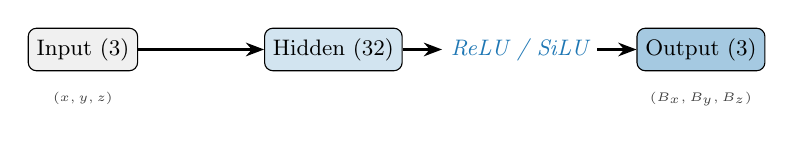
\begin{tikzpicture}[
    node distance=0.6cm and 1.6cm,
    layer/.style={draw, rounded corners=3pt, minimum width=1.3cm,
                  minimum height=0.6cm, font=\small},
    arrow/.style={-Stealth, thick},
    scale=0.9, every node/.style={scale=0.9}
  ]
    \node[layer, fill=lightgray] (in) {Input (3)};
    \node[below=0.15cm of in, font=\tiny, text=darkgray] {$(x, y, z)$};

    \node[layer, fill=lhcbblue!20, right=of in] (h1) {Hidden (32)};

    \node[right=0.5cm of h1, font=\small\itshape, text=lhcbblue] (act)
      {ReLU / SiLU};

    \node[layer, fill=lhcbblue!40, right=0.5cm of act] (out) {Output (3)};
    \node[below=0.15cm of out, font=\tiny, text=darkgray]
      {$(B_x, B_y, B_z)$};

    \draw[arrow] (in) -- (h1);
    \draw[arrow] (h1) -- (act);
    \draw[arrow] (act) -- (out);
  \end{tikzpicture}

  \vspace{10pt}
  \begin{tabular}{@{} l r @{}}
    \toprule
    \textbf{Property} & \textbf{Value} \\
    \midrule
    Parameters        & 227 \\
    Memory            & 908~bytes (float32) \\
    FLOPs (ReLU)      & 416 \\
    FLOPs (SiLU)      & 512 \\
    \bottomrule
  \end{tabular}
\end{column}

\begin{column}{0.46\textwidth}
  \textbf{Forward pass} with z-score normalisation:
  \begin{align*}
    \hat{\bvec{x}} &= \frac{\bvec{x} - \bvec{\mu}_\text{in}}
                          {\bvec{\sigma}_\text{in}} \\[4pt]
    \bvec{h} &= \sigma\bigl(W_1\,\hat{\bvec{x}} + \bvec{b}_1\bigr) \\[4pt]
    \hat{\bvec{y}} &= W_2\,\bvec{h} + \bvec{b}_2 \\[4pt]
    \bvec{B} &= \hat{\bvec{y}} \cdot \bvec{\sigma}_\text{out}
                + \bvec{\mu}_\text{out}
  \end{align*}

  \vspace{4pt}
  \textbf{Activations:}
  \begin{itemize}\small
    \item ReLU: $\sigma(x) = \max(0, x)$\\
          --- 1 FLOP/neuron, SIMD-friendly
    \item SiLU: $\sigma(x) = x/(1+e^{-x})$\\
          --- smoother, 4 FLOPs/neuron
  \end{itemize}
\end{column}
\end{columns}
\end{frame}


% =============================================================================
\begin{frame}{Grid Search: 30 Architectures}

\begin{columns}[T]
\begin{column}{0.48\textwidth}
  \textbf{Search space:}
  \begin{itemize}\small
    \item Hidden widths: 32, 64, 128, 256, 512
    \item Depths: 1, 2, 3 layers
    \item Activations: ReLU, SiLU
    \item $= 5 \times 3 \times 2 = 30$ models
  \end{itemize}

  \vspace{6pt}
  \textbf{Training:}
  \begin{itemize}\small
    \item Train on all 957{,}906 grid vertices
    \item Validate on 100K random off-grid points\\
          (ground truth = trilinear interpolation)
    \item Adam, cosine LR schedule, batch 4096
  \end{itemize}

  \vspace{6pt}
  \textbf{Accuracy targets:}
  \begin{itemize}\small
    \item MAE $< 0.1$~Gauss
    \item p99 $< 1.0$~Gauss
    \item Max $< 10.0$~Gauss
  \end{itemize}
\end{column}

\begin{column}{0.48\textwidth}
  \begin{figure}
    
\includegraphics[width=\textwidth]{pareto_accuracy_vs_flops.png}
    \caption*{\scriptsize Pareto frontier: accuracy vs computational cost.}
  \end{figure}
\end{column}
\end{columns}
\end{frame}


% =============================================================================
\begin{frame}{L1/L2 Cache Analysis --- The Key Speedup Mechanism}

\begin{columns}[T]
\begin{column}{0.52\textwidth}
  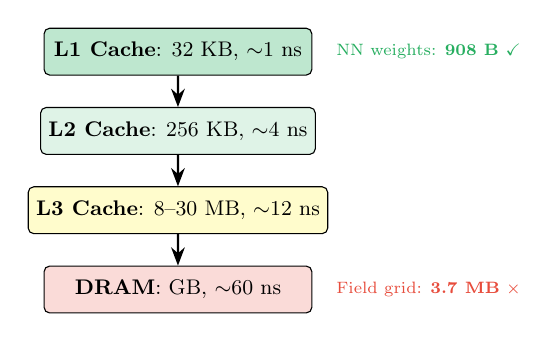
\begin{tikzpicture}[
    cache/.style={draw, minimum width=4cm, minimum height=0.7cm,
                  font=\small, align=center, rounded corners=2pt},
    scale=0.85, every node/.style={scale=0.85}
  ]
    % L1
    \node[cache, fill=cachegreen!30] (l1) at (0,0)
      {\textbf{L1 Cache}: 32~KB, $\sim$1~ns};
    \node[right=0.2cm of l1, font=\scriptsize, text=cachegreen]
      {NN weights: \textbf{908 B} $\checkmark$};

    % L2
    \node[cache, fill=cachegreen!15, below=0.4cm of l1] (l2)
      {\textbf{L2 Cache}: 256~KB, $\sim$4~ns};

    % L3
    \node[cache, fill=yellow!20, below=0.4cm of l2] (l3)
      {\textbf{L3 Cache}: 8--30~MB, $\sim$12~ns};

    % DRAM
    \node[cache, fill=cachered!20, below=0.4cm of l3] (dram)
      {\textbf{DRAM}: GB, $\sim$60~ns};
    \node[right=0.2cm of dram, font=\scriptsize, text=cachered]
      {Field grid: \textbf{3.7~MB} $\times$};

    % Arrows
    \draw[-Stealth, thick] (l1) -- (l2);
    \draw[-Stealth, thick] (l2) -- (l3);
    \draw[-Stealth, thick] (l3) -- (dram);
  \end{tikzpicture}
\end{column}

\begin{column}{0.46\textwidth}
  \textbf{Trilinear interpolation:}
  \begin{itemize}\small
    \item 8 corner lookups $\times$ 3 components
    \item Scattered access in $\sim$3.7~MB 3D grid
    \item Cache miss $\Rightarrow$ $\sim$60~ns latency
    \item Memory-bound, not compute-bound
  \end{itemize}

  \vspace{8pt}
  \textbf{NN field evaluation:}
  \begin{itemize}\small
    \item 227 parameters $\times$ 4 bytes $=$ \textbf{908~B}
    \item Fits \textbf{entirely} in L1 cache
    \item All accesses sequential (matrix--vector)
    \item Compute-bound (ALU-limited)
  \end{itemize}

  \vspace{8pt}
  \begin{exampleblock}{Key insight}
    The NN trades raw FLOP count (416 vs 57) for
    \textbf{cache locality}. With 69 field calls per track,
    the NN weights stay L1-resident throughout.
  \end{exampleblock}
\end{column}
\end{columns}
\end{frame}


% =============================================================================
\begin{frame}{Hot Cache vs Cold Cache --- Real-World Impact}

\begin{columns}[T]
\begin{column}{0.50\textwidth}
  \begin{table}
  \centering\scriptsize
  \begin{tabular}{@{} l r r r @{}}
    \toprule
    \textbf{Component} & \textbf{Hot} & \textbf{Cold} & \textbf{Cold/} \\
    & \textbf{(ns)} & \textbf{(ns)} & \textbf{Hot} \\
    \midrule
    \multicolumn{4}{@{}l}{\textit{Per-call field evaluation:}} \\
    Trilinear             & 106 & 740  & $7.0\times$ \\
    NN~[32] SiLU          & 318 & 1483 & $4.7\times$ \\
    NN~[32] ReLU          & 109 & 837  & $7.7\times$ \\
    NN~[32,32] ReLU       & 1014 & 1837 & $1.8\times$ \\
    \midrule
    \multicolumn{4}{@{}l}{\textit{Cash--Karp step (6 stages):}} \\
    Trilinear             & 545  & 1110 & $2.0\times$ \\
    NN~[32] SiLU          & 2146 & 3299 & $1.5\times$ \\
    NN~[32] ReLU          & 711  & 1557 & $2.2\times$ \\
    NN~[32,32] ReLU       & 5842 & 6625 & $1.1\times$ \\
    \bottomrule
  \end{tabular}
  \caption*{\scriptsize \textbf{C++ micro-benchmark}, \texttt{-O2}.\\
            Cold: 32~MB flush between calls.}
  \end{table}
\end{column}

\begin{column}{0.48\textwidth}
  \begin{figure}
    
\includegraphics[width=\textwidth]{cache_cold_per_step.pdf}
    \caption*{\scriptsize Hot vs cold cache timing per CK step.}
  \end{figure}

  \vspace{4pt}
  \begin{exampleblock}{Key observations}
    \begin{itemize}\scriptsize
      \item Trilinear: $7\times$ cold penalty (DRAM latency)
      \item CK step amortises: first call warms cache for remaining 5
      \item NN vs trilinear ratio is \emph{stable} hot or cold\\
            $\Rightarrow$ NN advantage survives in production
    \end{itemize}
  \end{exampleblock}
\end{column}
\end{columns}
\end{frame}


% =============================================================================
\begin{frame}[fragile]{AVX2 SIMD Implementation (1/2) --- Inner Loop}

Deployed in \texttt{FieldMapNNReLUWeights.h}. Process \textbf{8 neurons
simultaneously} using 256-bit AVX2 registers:

\vspace{2pt}
\begin{lstlisting}[language=C++, title={\scriptsize Pseudo-code (from LHCb stack implementation)}]
// Weights stored transposed: w[input][neuron_block] for coalesced loads
__m256 vin0 = _mm256_set1_ps(x_norm);   // broadcast normalised x
__m256 vin1 = _mm256_set1_ps(y_norm);   // broadcast normalised y
__m256 vin2 = _mm256_set1_ps(z_norm);   // broadcast normalised z

for (int blk = 0; blk < 4; ++blk) {    // 4 blocks x 8 = 32 neurons
  __m256 vh = _mm256_load_ps(&bias[blk*8]);         // load 8 biases
  vh = _mm256_fmadd_ps(w_x[blk], vin0, vh);         // + w_x * x
  vh = _mm256_fmadd_ps(w_y[blk], vin1, vh);         // + w_y * y
  vh = _mm256_fmadd_ps(w_z[blk], vin2, vh);         // + w_z * z
  vh = _mm256_max_ps(vh, _mm256_setzero_ps());       // ReLU

  // Accumulate into 3 output neurons
  for (int j = 0; j < 3; ++j)
    acc[j] = _mm256_fmadd_ps(out_w[j][blk], vh, acc[j]);
}
// Horizontal sum: acc[j] -> scalar via _mm256_hadd_ps chain
\end{lstlisting}

\vspace{2pt}
\begin{itemize}\small
  \item \textbf{3 FMAs + 1 max} per block = 4 SIMD instructions for 8 neurons
  \item Transposed weight layout eliminates gather operations
  \item All weights stay in registers / L1 across all 69 calls per track
\end{itemize}
\end{frame}


% =============================================================================
\begin{frame}[fragile]{AVX2 SIMD Implementation (2/2) --- Batch Mode}

\texttt{evaluate\_relu\_avx2\_batch<N>}: processes $N$ tracks with
\textbf{shared weight register loads}:

\begin{lstlisting}[language=C++, title={\scriptsize Batch pseudo-code}]
template<int N>
void evaluate_relu_avx2_batch(const float inputs[N][3],
                               float outputs[N][3]) {
  for (int blk = 0; blk < 4; ++blk) {
    // Load weights ONCE per block (shared across N tracks)
    __m256 vw0 = _mm256_load_ps(&w_x[blk*8]);
    __m256 vw1 = _mm256_load_ps(&w_y[blk*8]);
    __m256 vw2 = _mm256_load_ps(&w_z[blk*8]);
    __m256 vb  = _mm256_load_ps(&bias[blk*8]);

    for (int t = 0; t < N; ++t) {         // Per-track evaluation
      __m256 vh = _mm256_fmadd_ps(vw0, broadcast(inputs[t][0]), vb);
      vh = _mm256_fmadd_ps(vw1, broadcast(inputs[t][1]), vh);
      vh = _mm256_fmadd_ps(vw2, broadcast(inputs[t][2]), vh);
      vh = _mm256_max_ps(vh, zero);        // ReLU
      accumulate_outputs(t, blk, vh);      // output FMAs
    }
  }
}
\end{lstlisting}

\vspace{2pt}
\begin{columns}[T]
\begin{column}{0.48\textwidth}
  \textbf{NN (ALU-bound):}
  \begin{itemize}\scriptsize
    \item Weight loads amortised over $N$ tracks
    \item Predictable, sequential access
    \item Fully utilises FMA pipeline
  \end{itemize}
\end{column}
\begin{column}{0.48\textwidth}
  \textbf{Trilinear (memory-bound):}
  \begin{itemize}\scriptsize
    \item 8 gather ops per call (scattered)
    \item Cache thrashing for $N > 1$ tracks
    \item SIMD divergence on boundary checks
  \end{itemize}
\end{column}
\end{columns}
\end{frame}


% =============================================================================
\begin{frame}{$-$O2 / $-$O3 Compiler Optimisation Effects}

\begin{table}
\centering\small
\begin{tabular}{@{} p{2.4cm} p{4.8cm} p{4.8cm} @{}}
  \toprule
  \textbf{Feature} & \textbf{Effect on NN field eval} &
    \textbf{Effect on trilinear interp.} \\
  \midrule
  \texttt{-O2} baseline &
    Standard inlining; loop opt &
    Standard inlining; branch pred. \\[4pt]
  \texttt{-O3} auto-vectorise &
    Small function body (227 params) $\Rightarrow$ \textbf{fully inlined \&
    unrolled} &
    Branch-heavy logic $\Rightarrow$ limited vectorisation benefit \\[4pt]
  Loop unrolling &
    4-iteration hidden-layer loop fully unrolled &
    Boundary checks prevent full unrolling \\[4pt]
  FMA fusion &
    $W\bvec{x}+\bvec{b}$ maps directly to \texttt{fmadd} &
    Scattered multiply-add patterns; less FMA opportunity \\[4pt]
  \texttt{-ffast-math} &
    Enables reciprocal $\sqrt{}$ approx for SiLU &
    Minimal benefit (no transcendentals) \\
  \bottomrule
\end{tabular}
\end{table}

\vspace{6pt}
\begin{block}{Butcher accumulation in the RK stepper}
  \texttt{std::transform\_reduce(..., std::execution::unseq, ...)}\\
  $\Rightarrow$ auto-vectorised by the compiler under \texttt{-O3}
\end{block}
\end{frame}


% =============================================================================
\begin{frame}{Measured Cycle Costs: Component Breakdown}

\begin{columns}[T]
\begin{column}{0.50\textwidth}
  \begin{table}
  \centering\scriptsize
  \begin{tabular}{@{} l r r r @{}}
    \toprule
    \textbf{Component} & \textbf{\texttt{-O2}} & \textbf{\texttt{-O3}} &
      \textbf{vs.\ trilinear} \\
    & \textbf{(ns)} & \textbf{(ns)} & \textbf{(\texttt{-O3})} \\
    \midrule
    Trilinear interp.   & 106 & 116 & $1.0\times$ \\
    NN~[32] SiLU        & 318 & 139 & $0.83\times$ \\
    NN~[32] ReLU        & 109 & 40  & $\bvec{2.9\times}$ \\
    NN~[32,32] ReLU     & ---  & 155 & $0.75\times$ \\
    Lorentz derivative  & 17  & 11  & --- \\
    \bottomrule
  \end{tabular}
  \caption*{\scriptsize Per-call field evaluation.\\
            {\color{darkgray}\textbf{C++ micro-benchmark}, 100K iterations,
            AMD EPYC~7551P.}}
  \end{table}

  \vspace{2pt}
  \begin{table}
  \centering\scriptsize
  \begin{tabular}{@{} l r r @{}}
    \toprule
    \textbf{Component} & \textbf{FLOPs/step} & \textbf{Fraction} \\
    \midrule
    B-field ($6\times56$)     & 336  & 60.2\% \\
    Lorentz deriv ($6\times17$)& 102 & 18.3\% \\
    Butcher bookkeeping       & 120  & 21.5\% \\
    \midrule
    \textbf{Simplified step}  & \textbf{558} & 100\% \\
    \bottomrule
  \end{tabular}
  \caption*{\scriptsize FLOP decomposition of a single CK step\\
            (micro-benchmark scope, no Jacobian).}
  \end{table}
\end{column}

\begin{column}{0.48\textwidth}
  \begin{figure}
    
\includegraphics[width=\textwidth]{cashkarp_step_breakdown.pdf}
    \caption*{\scriptsize CK step breakdown: FLOPs (left) and
              measured timing per field method (right).}
  \end{figure}

  \vspace{4pt}
  \begin{alertblock}{SiLU bottleneck}
    32 \texttt{exp()} calls = 80\% of SiLU inference cost.\\
    Switching to ReLU: $2.9\times$ faster at \texttt{-O3}.
  \end{alertblock}
\end{column}
\end{columns}
\end{frame}


% =============================================================================
\begin{frame}{Optimisation Progression: CK Step Timing}

\begin{columns}[T]
\begin{column}{0.50\textwidth}
  \begin{table}
  \centering\scriptsize
  \begin{tabular}{@{} l r r r @{}}
    \toprule
    \textbf{Variant} & \textbf{\texttt{-O2}} & \textbf{\texttt{-O3}} &
      \textbf{vs.\ trilinear} \\
    & \textbf{(ns)} & \textbf{(ns)} & \textbf{(\texttt{-O3})} \\
    \midrule
    Trilinear           & 545 & 331 & $1.00\times$ \\
    NN scalar ReLU      & 711 & 264 & $0.80\times$ \\
    NN batch-6          & 623 & 157 & $0.47\times$ \\
    NN AVX2 (gathered)  & 933 & 376 & $1.14\times$ \\
    NN AVX2 (aligned)   & 265 & 198 & $0.60\times$ \\
    NN unrolled         & 826 & 644 & $1.94\times$ \\
    \rowcolor{nngreen!15}
    \textbf{NN AVX2 batch-6} & \textbf{254} & \textbf{58} &
      $\bvec{0.17\times}$ \\
    \bottomrule
  \end{tabular}
  \caption*{\scriptsize CK step (6 stages, simplified kernel).\\
            {\color{darkgray}\textbf{C++ micro-benchmark}, 100K iterations.}}
  \end{table}

  \vspace{2pt}
  \begin{alertblock}{Failed optimisations}
    \begin{itemize}\scriptsize
      \item AVX2 gathered (no pre-transposition): \textbf{slower}
      \item Manual unrolling: $2\times$ \textbf{slower}
    \end{itemize}
  \end{alertblock}
\end{column}

\begin{column}{0.48\textwidth}
  \begin{figure}
    
\includegraphics[width=\textwidth]{ck_step_optimisation_progression.pdf}
    \caption*{\scriptsize CK step timing: optimisation progression.\\
              Trilinear baseline shown as dashed line.}
  \end{figure}

  \vspace{2pt}
  \begin{exampleblock}{$5.7\times$ CK step speedup}
    AVX2 batch-6: 58~ns vs 331~ns (trilinear).\\
    Exceeds Amdahl bound ($2.5\times$) because\\
    batching restructures the \emph{entire} step.
  \end{exampleblock}
\end{column}
\end{columns}
\end{frame}


% =============================================================================
\begin{frame}{Full Track Timing \& Production Comparison}

\begin{columns}[T]
\begin{column}{0.50\textwidth}
  \begin{table}
  \centering\scriptsize
  \begin{tabular}{@{} l r r r @{}}
    \toprule
    \textbf{Variant} & \textbf{\texttt{-O2}} & \textbf{\texttt{-O3}} &
      \textbf{vs.\ trilinear} \\
    & \textbf{(ns)} & \textbf{(ns)} & \textbf{(\texttt{-O3})} \\
    \midrule
    Trilinear          & 2916 & 2141 & $1.00\times$ \\
    NN scalar ReLU     & 6658 & 3180 & $1.49\times$ \\
    NN batch-6         & 5813 & 1448 & $0.68\times$ \\
    NN AVX2 (aligned)  & 2520 & 2016 & $0.94\times$ \\
    \rowcolor{nngreen!15}
    \textbf{NN AVX2 batch-6} & \textbf{2375} & \textbf{427} &
      $\bvec{0.20\times}$ \\
    \bottomrule
  \end{tabular}
  \caption*{\scriptsize 10 simplified CK steps, $z{=}3000{\to}7000$~mm.\\
            {\color{darkgray}\textbf{C++ micro-benchmark},
            no Jacobian/adaptive stepping.}}
  \end{table}

  \vspace{2pt}
  \begin{figure}
    
\includegraphics[width=\textwidth]{full_track_optimised_comparison.pdf}
    \caption*{\scriptsize Full track: all NN variants vs trilinear.}
  \end{figure}
\end{column}

\begin{column}{0.48\textwidth}
  \begin{table}
  \centering\scriptsize
  \begin{tabular}{@{} l r r @{}}
    \toprule
    \textbf{Extrapolator} & \textbf{Time} & \textbf{Pos.\ err} \\
    & \textbf{($\mu$s)} & \textbf{(mm)} \\
    \midrule
    CashKarp RK5(4)       & 2.50 & 0.00 \\
    Bogacki--Shampine~3   & 2.40 & 0.10 \\
    Verner RK9(8)         & 2.52 & 0.08 \\
    Tsitouras RK5(4)      & 2.75 & --- \\
    Herab RK5             & 1.95 & 5.10 \\
    Kisel polynomial      & 1.50 & 39.8 \\
    \bottomrule
  \end{tabular}
  \caption*{\scriptsize {\color{rk4red}\textbf{Full Gaudi/QMTest benchmark}}:\\
            RDTSC clock, 121-track grid, $z{=}3000{\to}7000$~mm.\\
            Includes Jacobian, adaptive stepping, covariance.}
  \end{table}

  \vspace{2pt}
  \begin{figure}
    
\includegraphics[width=\textwidth]{extrapolator_timing_comparison.pdf}
    \caption*{\scriptsize Production extrapolator comparison (QMTest).}
  \end{figure}
\end{column}
\end{columns}
\end{frame}


% =============================================================================
\begin{frame}{Field NN Results: Accuracy \& Speed}

\begin{columns}[T]
\begin{column}{0.48\textwidth}
  \begin{figure}
    
\includegraphics[width=\textwidth]{per_component_errors.png}
    \caption*{\scriptsize Per-component field errors ($B_x$, $B_y$, $B_z$).}
  \end{figure}
\end{column}

\begin{column}{0.48\textwidth}
  \begin{figure}
    
\includegraphics[width=\textwidth]{v2_batched_speedup.png}
    \caption*{\scriptsize Batched inference throughput comparison.}
  \end{figure}
\end{column}
\end{columns}

\end{frame}


% #############################################################################
\section{Neural Network Full Extrapolation}
% #############################################################################

% =============================================================================
\begin{frame}{Strategy: Replace the Entire RK Step}

\begin{block}{Concept}
  Train a neural network to learn the \textbf{full input--output mapping}
  of the Runge--Kutta integrator in a single forward pass.
\end{block}

\vspace{6pt}
\textbf{Input} (6 features):
\begin{equation*}
  \bvec{x}_\text{in} = \bigl(\,x_0,\; y_0,\; \tx{}_0,\; \ty{}_0,\;
  \qop,\; \dz\,\bigr)
\end{equation*}

\textbf{Output} (4 features):
\begin{equation*}
  \bvec{x}_\text{out} = \bigl(\,x,\; y,\; \tx,\; \ty\,\bigr)
  \quad\text{at}\quad z = z_0 + \dz
\end{equation*}

\vspace{6pt}
\textbf{Training data}: 50--100M trajectories generated by CashKarp RK4
integration through the real LHCb dipole field map.

\vspace{6pt}
\textbf{Best approach found}: a simple \textbf{multi-layer perceptron (MLP)}
with SiLU activation and supervised MSE loss --- no physics-informed
constraints needed.
\end{frame}


% =============================================================================
\begin{frame}{MLP Extrapolator Architecture}

\begin{columns}[T]
\begin{column}{0.52\textwidth}
  \centering
  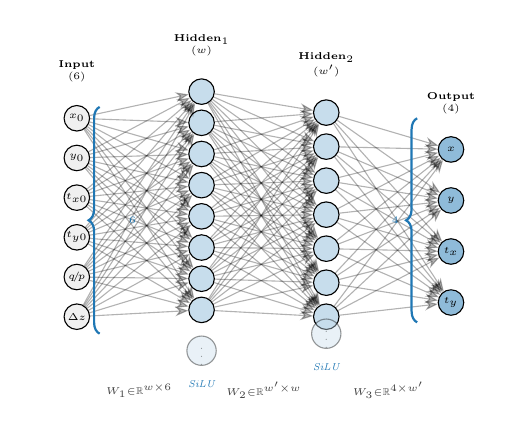
\begin{tikzpicture}[
    neuron/.style={draw, circle, minimum size=0.45cm, inner sep=0pt,
                   font=\tiny},
    input neuron/.style={neuron, fill=lightgray},
    hidden neuron/.style={neuron, fill=lhcbblue!25},
    output neuron/.style={neuron, fill=lhcbblue!50},
    annot/.style={text width=1.5cm, align=center, font=\tiny},
    arrow/.style={-Stealth, thin, opacity=0.3},
    scale=0.72, every node/.style={scale=0.72}
  ]
    % Input layer (explicit nodes to avoid foreach delimiter issues)
    \node[input neuron] (I-1) at (0,-0.7)  {$x_0$};
    \node[input neuron] (I-2) at (0,-1.4)  {$y_0$};
    \node[input neuron] (I-3) at (0,-2.1)  {$t_{x0}$};
    \node[input neuron] (I-4) at (0,-2.8)  {$t_{y0}$};
    \node[input neuron] (I-5) at (0,-3.5)  {$q\!/\!p$};
    \node[input neuron] (I-6) at (0,-4.2)  {$\Delta z$};
    \node[annot, above=0.2cm of I-1] {\textbf{Input}\\(6)};

    % Hidden 1
    \foreach \i in {1,...,8}
      \node[hidden neuron] (H1-\i) at (2.2,-\i*0.55+0.32) {};
    \node[hidden neuron, opacity=0.4] (H1-d) at (2.2,-4.8) {$\vdots$};
    \node[annot, above=0.2cm of H1-1] {\textbf{Hidden$_1$}\\($w$)};
    \node[below=0.1cm of H1-d, font=\tiny\itshape, text=lhcbblue]
      {SiLU};

    % Hidden 2
    \foreach \i in {1,...,7}
      \node[hidden neuron] (H2-\i) at (4.4,-\i*0.6+0.0) {};
    \node[hidden neuron, opacity=0.4] (H2-d) at (4.4,-4.5) {$\vdots$};
    \node[annot, above=0.2cm of H2-1] {\textbf{Hidden$_2$}\\($w'$)};
    \node[below=0.1cm of H2-d, font=\tiny\itshape, text=lhcbblue]
      {SiLU};

    % Output layer (explicit nodes)
    \node[output neuron] (O-1) at (6.6,-1.25) {$x$};
    \node[output neuron] (O-2) at (6.6,-2.15) {$y$};
    \node[output neuron] (O-3) at (6.6,-3.05) {$t_x$};
    \node[output neuron] (O-4) at (6.6,-3.95) {$t_y$};
    \node[annot, above=0.2cm of O-1] {\textbf{Output}\\(4)};

    % Connections Input -> H1
    \foreach \i in {1,...,6}
      \foreach \j in {1,...,8}
        \draw[arrow] (I-\i) -- (H1-\j);

    % Connections H1 -> H2
    \foreach \i in {1,...,8}
      \foreach \j in {1,...,7}
        \draw[arrow] (H1-\i) -- (H2-\j);

    % Connections H2 -> Output
    \foreach \i in {1,...,7}
      \foreach \j in {1,...,4}
        \draw[arrow] (H2-\i) -- (O-\j);

    % Dimension annotations
    \draw[decorate, decoration={brace, amplitude=4pt, mirror, raise=2pt},
          thick, lhcbblue]
      (0.5,-0.5) -- (0.5,-4.5) node[midway, right=6pt, font=\tiny] {6};
    \draw[decorate, decoration={brace, amplitude=4pt, mirror, raise=2pt},
          thick, lhcbblue]
      (6.1,-0.7) -- (6.1,-4.3) node[midway, left=6pt, font=\tiny] {4};

    % Weight matrix labels
    \node[font=\tiny, text=darkgray] at (1.1,-5.5) {$W_1{\in}\mathbb{R}^{w\times6}$};
    \node[font=\tiny, text=darkgray] at (3.3,-5.5) {$W_2{\in}\mathbb{R}^{w'\times w}$};
    \node[font=\tiny, text=darkgray] at (5.5,-5.5) {$W_3{\in}\mathbb{R}^{4\times w'}$};
  \end{tikzpicture}
\end{column}

\begin{column}{0.46\textwidth}
  \textbf{Forward pass} (with z-score normalisation):
  \begin{align*}
    \hat{\bvec{x}} &= \frac{\bvec{x}_\text{in} - \bvec{\mu}}
                          {\bvec{\sigma}} \\[3pt]
    \bvec{h}_1 &= \sigma(W_1\,\hat{\bvec{x}} + \bvec{b}_1) \\[3pt]
    \bvec{h}_2 &= \sigma(W_2\,\bvec{h}_1 + \bvec{b}_2) \\[3pt]
    \hat{\bvec{y}} &= W_3\,\bvec{h}_2 + \bvec{b}_3
  \end{align*}

  where $\sigma(x) = x/(1+e^{-x})$ (SiLU).

  \vspace{6pt}
  \textbf{Architecture presets:}
  \begin{table}
  \centering\scriptsize
  \begin{tabular}{@{} l c r @{}}
    \toprule
    \textbf{Name} & \textbf{Layers} & \textbf{Params} \\
    \midrule
    single\_256       & [256]         & $\sim$1.5K \\
    single\_512       & [512]         & $\sim$3K \\
    shallow\_256      & [256, 256]    & $\sim$101K \\
    \textbf{shallow\_512\_256} & \textbf{[512, 256]} & $\sim$\textbf{402K} \\
    medium            & [256, 256, 128] & $\sim$100K \\
    wide              & [512, 512, 256, 128] & $\sim$500K \\
    \bottomrule
  \end{tabular}
  \end{table}
\end{column}
\end{columns}
\end{frame}


% =============================================================================
\begin{frame}{Training \& Loss Function}

\begin{columns}[T]
\begin{column}{0.52\textwidth}
  \textbf{Loss function} --- pure supervised MSE:
  \begin{equation*}
    \boxed{\;
    \mathcal{L}(\theta) = \frac{1}{B}\sum_{i=1}^{B}
    \bigl\|\hat{\bvec{y}}_i(\theta) - \bvec{y}_i^\text{RK4}\bigr\|^2
    \;}
  \end{equation*}

  \vspace{4pt}
  Expanded over output components:
  \begin{equation*}
    \mathcal{L} = \frac{1}{B}\sum_{i=1}^{B}\Bigl[
      (\hat{x}_i - x_i)^2 + (\hat{y}_i - y_i)^2
      + (\hat{\tx}_i - \tx{}_i)^2 + (\hat{\ty}_i - \ty{}_i)^2
    \Bigr]
  \end{equation*}

  \vspace{6pt}
  \textbf{Why MSE?}
  \begin{itemize}\small
    \item Targets $\bvec{y}^\text{RK4}$ are generated by CashKarp RK4\\
          $\Rightarrow$ clean labels, no noise
    \item No physics-informed regularisation needed:\\
          the data \emph{already encodes} the physics
    \item Simpler = faster convergence, no hyperparameter
          balancing between loss terms
  \end{itemize}
\end{column}

\begin{column}{0.46\textwidth}
  \textbf{Training configuration:}
  \begin{table}
  \centering\scriptsize
  \begin{tabular}{@{} l l @{}}
    \toprule
    \textbf{Parameter} & \textbf{Value} \\
    \midrule
    Optimiser        & Adam ($\beta_1{=}0.9$, $\beta_2{=}0.999$) \\
    Learning rate    & $10^{-3}$ (initial) \\
    LR schedule      & Cosine annealing to $10^{-5}$ \\
    Batch size       & 2048 \\
    Epochs           & 100 (early stopping) \\
    Training samples & 50--100M RK4 trajectories \\
    Validation split & 10\% \\
    Activation       & SiLU \\
    Weight init      & Kaiming uniform \\
    \bottomrule
  \end{tabular}
  \end{table}

  \vspace{4pt}
  \textbf{Data generation:}
  \begin{itemize}\scriptsize
    \item Sample $(x_0, y_0, \tx{}_0, \ty{}_0, \qop, \dz)$
          uniformly from the physical domain
    \item Propagate with CashKarp RK4 through the real
          LHCb dipole field map to obtain $\bvec{y}^\text{RK4}$
    \item Z-score normalise inputs \emph{and} outputs
  \end{itemize}
\end{column}
\end{columns}
\end{frame}


% =============================================================================
\begin{frame}{Architecture Selection: Shallow--Wide Wins}

\begin{columns}[T]
\begin{column}{0.48\textwidth}
  \begin{figure}
    
\includegraphics[width=\textwidth]{mlp_width_depth_comparison.png}
    \caption*{\scriptsize MLP width $\times$ depth comparison across
              100+ trained models.}
  \end{figure}
\end{column}

\begin{column}{0.50\textwidth}
  \textbf{Key finding:}

  \vspace{4pt}
  2-layer networks with 256--512 neurons \textbf{consistently outperform}
  5-layer networks with 64 neurons --- both in accuracy and inference speed.

  \vspace{8pt}
  \textbf{Why?}
  \begin{itemize}\small
    \item Shallow-wide: large matrix--vector products that saturate SIMD
    \item Deep-narrow: many small sequential operations, poor ILP
    \item The extrapolation mapping is smooth $\Rightarrow$ a wide single
          layer captures most of the variation
  \end{itemize}

  \vspace{8pt}
  \begin{exampleblock}{Best architecture}
    \textbf{[512, 256]} (2 hidden layers)\\
    402K params, 0.028~mm position error\\
    1.93~$\mu$s inference, 1.3$\times$ faster than RK4
  \end{exampleblock}
\end{column}
\end{columns}
\end{frame}


% =============================================================================
\begin{frame}{Results: Fixed $\dz = 8000$~mm}

\begin{columns}[T]
\begin{column}{0.48\textwidth}
  \begin{table}
  \centering\small
  \begin{tabular}{@{} l r r r @{}}
    \toprule
    \textbf{Model} & \textbf{Pos.} & \textbf{Time} &
      \textbf{Speedup} \\
    & \textbf{(mm)} & \textbf{($\mu$s)} & \\
    \midrule
    \rowcolor{nngreen!10}
    single\_256    & 0.065 & 0.83 & \textbf{3.0$\times$} \\
    \rowcolor{nngreen!10}
    shallow\_256   & 0.044 & 1.50 & 1.7$\times$ \\
    \rowcolor{nngreen!15}
    \textbf{shallow\_512\_256} & \textbf{0.028} & \textbf{1.93} &
      \textbf{1.3$\times$} \\
    shallow\_1024\_256 & 0.031 & 3.56 & 0.7$\times$ \\
    \midrule
    C++ RK4        & 0     & 2.50 & 1.0$\times$ \\
    \bottomrule
  \end{tabular}
  \caption*{\scriptsize V2 benchmark: MLP vs C++ CashKarp RK4.\\
            Position error = mean RMSE across test set.}
  \end{table}
\end{column}

\begin{column}{0.50\textwidth}
  \begin{figure}
    
\includegraphics[width=\textwidth]{speed_vs_accuracy.png}
    \caption*{\scriptsize Speed vs accuracy Pareto frontier.}
  \end{figure}

  \vspace{2pt}
  \begin{block}{Key results}
    \begin{itemize}\small
      \item \textbf{0.028~mm} position accuracy at \textbf{1.3$\times$}
            speedup
      \item \textbf{0.065~mm} at \textbf{3.0$\times$} speedup
      \item Sub-100$\mu$m accuracy across the board
    \end{itemize}
  \end{block}
\end{column}
\end{columns}
\end{frame}


% =============================================================================
\begin{frame}{Results: Variable $\dz \in [500, 12000]$~mm}

\begin{columns}[T]
\begin{column}{0.48\textwidth}
  \begin{table}
  \centering\small
  \begin{tabular}{@{} l r r r @{}}
    \toprule
    \textbf{Model} & \textbf{Params} & \textbf{Time} & \textbf{Pos.} \\
    & & \textbf{($\mu$s)} & \textbf{RMSE} \\
    \midrule
    RK4 (truth)    & ---   & 85.2  & 0 \\
    Linear         & ---   & 0.04  & 1.63~mm \\
    Parabolic      & ---   & 0.09  & 1.63~mm \\
    \midrule
    \rowcolor{nngreen!10}
    MLP deep\_128  & 59K   & 65.0  & 1.01~mm \\
    \rowcolor{nngreen!10}
    MLP shallow\_256 & 101K & 116.2 & 1.01~mm \\
    MLP deep\_256   & 233K & 265.7 & 1.06~mm \\
    MLP shallow\_512 & 399K & 465.6 & 0.96~mm \\
    \bottomrule
  \end{tabular}
  \caption*{\scriptsize V3 C++ single-sample benchmark.\\
            Variable $\dz$ is $\sim$35$\times$ harder than fixed.}
  \end{table}
\end{column}

\begin{column}{0.50\textwidth}
  \begin{figure}
    
\includegraphics[width=\textwidth]{component_accuracy.png}
    \caption*{\scriptsize Per-component accuracy: $x$, $y$, $\tx$, $\ty$.}
  \end{figure}

  \vspace{2pt}
  \begin{alertblock}{Variable $\dz$ challenge}
    Position RMSE: 0.028~mm (fixed) $\to$ $\sim$1~mm (variable)\\
    = \textbf{35$\times$ harder} --- the network must learn
    step-size--dependent curvature.
  \end{alertblock}
\end{column}
\end{columns}
\end{frame}


% =============================================================================
\begin{frame}{Error Analysis}

\begin{columns}[T]
\begin{column}{0.48\textwidth}
  \begin{figure}
    
\includegraphics[width=\textwidth]{error_vs_kinematics.png}
    \caption*{\scriptsize Error vs kinematic variables (momentum, angles).}
  \end{figure}
\end{column}

\begin{column}{0.48\textwidth}
  \begin{figure}
    
\includegraphics[width=\textwidth]{error_distributions.png}
    \caption*{\scriptsize Residual distributions for the best MLP.}
  \end{figure}
\end{column}
\end{columns}

\vspace{2pt}
\begin{itemize}\small
  \item Low-momentum tracks ($p < 5$~GeV) have larger errors due to
        stronger bending --- the mapping is more nonlinear
  \item Error distributions are approximately Gaussian with zero mean\\
        $\Rightarrow$ no systematic bias
  \item Slope accuracy ($\tx$, $\ty$) is excellent: RMSE $\sim 0.007$~mrad
\end{itemize}
\end{frame}


% =============================================================================
\begin{frame}{C++ Deployment}

\begin{columns}[T]
\begin{column}{0.52\textwidth}
  \textbf{Inference engine}: \texttt{TrackMLPExtrapolator}
  \begin{itemize}\small
    \item \textbf{Eigen}-based matrix operations
    \item No TensorFlow / PyTorch dependency
    \item Supports ReLU, SiLU, Tanh, Sigmoid
    \item Input/output normalisation baked into model
  \end{itemize}

  \vspace{6pt}
  \textbf{Binary model format} (\texttt{.bin}):
  \begin{enumerate}\scriptsize
    \item Header: model type, number of layers
    \item Normalisation: input/output mean \& std
    \item Per-layer: weight matrix + bias vector (float64)
    \item Activation function name string
  \end{enumerate}

  \vspace{6pt}
  \textbf{Gaudi integration}:
  \begin{itemize}\small
    \item Configured via \texttt{ModelPath} property
    \item Drop-in replacement for \texttt{TrackRungeKuttaExtrapolator}
    \item Safety guards: max slope, max transverse position
  \end{itemize}
\end{column}

\begin{column}{0.46\textwidth}
  \textbf{QMTest validation pipeline:}

  \vspace{4pt}
  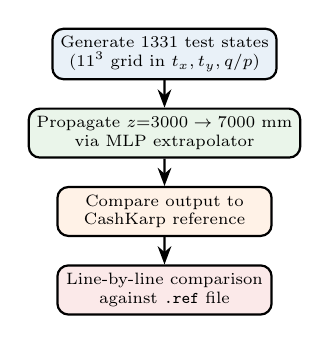
\begin{tikzpicture}[
    box/.style={draw, rounded corners, minimum width=3.2cm,
                minimum height=0.55cm, align=center, font=\scriptsize},
    >=Stealth, thick, scale=0.85, every node/.style={scale=0.85}
  ]
    \node[box, fill=lhcbblue!10] (gen) at (0,0)
      {Generate 1331 test states\\($11^3$ grid in $\tx,\ty,\qop$)};
    \node[box, fill=nngreen!10, below=0.35cm of gen] (prop)
      {Propagate $z{=}3000\to7000$~mm\\via MLP extrapolator};
    \node[box, fill=rkorange!10, below=0.35cm of prop] (ref)
      {Compare output to\\CashKarp reference};
    \node[box, fill=rk4red!10, below=0.35cm of ref] (val)
      {Line-by-line comparison\\against \texttt{.ref} file};

    \draw[->] (gen) -- (prop);
    \draw[->] (prop) -- (ref);
    \draw[->] (ref) -- (val);
  \end{tikzpicture}

  \vspace{6pt}
  \begin{block}{Platform support}
    Architecture-specific reference files\\
    for x86\_64, ARM, optimised builds.
  \end{block}
\end{column}
\end{columns}
\end{frame}


% #############################################################################
\section{Summary \& Outlook}
% #############################################################################

% =============================================================================
\begin{frame}{Summary: Two Complementary Strategies}

\begin{table}
\centering\small
\begin{tabular}{@{} l c c c c @{}}
  \toprule
  \textbf{Approach} & \textbf{Accuracy} & \textbf{Speed} &
    \textbf{Status} & \textbf{Upgrade~II} \\
  \midrule
  Trilinear + RK4 &
    exact (ref) & 8.35~$\mu$s & Current production &
    \textcolor{cachered}{Too slow} \\[4pt]
  \textcolor{nngreen}{\textbf{NN field}} + RK4 &
    sub-Gauss &  cache speedup &
    Deployed in stack &
    \textcolor{cachegreen}{Ready} \\[4pt]
  \textcolor{lhcbblue}{\textbf{MLP}} (fixed $\dz$) &
    0.028~mm & 1.93~$\mu$s &
    Validated &
    \textcolor{cachegreen}{Promising} \\[4pt]
  \textcolor{lhcbblue}{\textbf{MLP}} (variable $\dz$) &
    $\sim$1~mm & $\sim$65~$\mu$s &
    Under optimisation &
    \textcolor{rkorange}{In progress} \\
  \bottomrule
\end{tabular}
\end{table}

\vspace{6pt}
\begin{columns}[T]
\begin{column}{0.48\textwidth}
  \textbf{NN field map surrogate:}
  \begin{itemize}\small
    \item 227-parameter MLP fits in L1 cache
    \item AVX2 SIMD: 8 neurons/cycle
    \item Sub-Gauss accuracy, negligible track impact
    \item Directly accelerates existing RK4 pipeline
  \end{itemize}
\end{column}
\begin{column}{0.48\textwidth}
  \textbf{MLP full extrapolation:}
  \begin{itemize}\small
    \item Simple feedforward architecture
    \item 0.028~mm at 1.3$\times$ speedup (fixed $\dz$)
    \item Shallow-wide $>$ deep-narrow
    \item Variable $\dz$ is 35$\times$ harder --- active R\&D
  \end{itemize}
\end{column}
\end{columns}
\end{frame}


% =============================================================================
\begin{frame}{Outlook: Towards Upgrade~II Readiness}

\begin{enumerate}
  \item \textbf{NN field map $\to$ production}
  \begin{itemize}\small
    \item Integrate best architecture into Gaudi field service
    \item Quantify real-event throughput improvement
    \item Validate with full reconstruction chain
  \end{itemize}

  \vspace{4pt}
  \item \textbf{MLP extrapolation: sub-mm at variable $\dz$}
  \begin{itemize}\small
    \item V5 architecture sweep: wider networks, alternative activations
    \item Momentum-binned specialists vs single universal model
    \item Target: $< 0.5$~mm position RMSE at all step sizes
  \end{itemize}

  \vspace{4pt}
  \item \textbf{Batched \& SIMD inference for C++}
  \begin{itemize}\small
    \item Apply AVX2 techniques from field NN to full extrapolator
    \item Batch multiple tracks for matrix--matrix operations
    \item Target: $< 1~\mu$s single-track inference
  \end{itemize}

  \vspace{4pt}
  \item \textbf{Material corrections integration}
  \begin{itemize}\small
    \item How to combine NN extrapolation with multiple scattering \& $dE/dx$?
    \item Hybrid approach: NN for field propagation + analytic material
  \end{itemize}
\end{enumerate}
\end{frame}


% =============================================================================
% BACKUP SLIDES
% =============================================================================
\appendix

\begin{frame}[plain]
  \centering
  {\Huge\textbf{Backup Slides}}
\end{frame}


% =============================================================================
\begin{frame}{Backup: Normalisation Constants (Field NN)}

\begin{table}
\centering\small
\begin{tabular}{@{} l r r @{}}
  \toprule
  & \textbf{Mean} & \textbf{Std} \\
  \midrule
  $x$ (mm) & 0.0 & 2338.09 \\
  $y$ (mm) & 0.0 & 2338.09 \\
  $z$ (mm) & 6749.9995 & 4214.56 \\
  \midrule
  $B_x$ (Gauss) & 0.0 & 22.147 \\
  $B_y$ (Gauss) & 0.12293 & 71.609 \\
  $B_z$ (Gauss) & 0.0 & 22.147 \\
  \bottomrule
\end{tabular}
\caption*{\scriptsize Z-score normalisation constants for the deployed
          field NN (3$\to$32$\to$3 ReLU).}
\end{table}
\end{frame}


% =============================================================================
\begin{frame}{Backup: V2 Full MLP Results Table}

\begin{table}
\centering\scriptsize
\begin{tabular}{@{} l c r r r r @{}}
  \toprule
  \textbf{Model} & \textbf{Architecture} & \textbf{Pos Mean} &
    \textbf{Pos 90th} & \textbf{Slope} & \textbf{Time} \\
  & & \textbf{(mm)} & \textbf{(mm)} & \textbf{(mrad)} & \textbf{($\mu$s)} \\
  \midrule
  shallow\_1024\_256 & [1024, 256] & 0.031 & 0.060 & 0.678 & 3.56 \\
  \rowcolor{nngreen!10}
  \textbf{shallow\_512\_256} & \textbf{[512, 256]} & \textbf{0.028} &
    \textbf{0.051} & \textbf{0.416} & \textbf{1.93} \\
  shallow\_512       & [512, 512]  & 0.029 & 0.053 & 0.333 & 2.58 \\
  shallow\_1024\_512 & [1024, 512] & 0.034 & 0.063 & 0.783 & 4.71 \\
  shallow\_256       & [256, 256]  & 0.044 & 0.087 & 0.263 & 1.50 \\
  single\_1024       & [1024]      & 0.062 & 0.149 & 0.026 & 1.86 \\
  \rowcolor{nngreen!10}
  \textbf{single\_256} & \textbf{[256]} & \textbf{0.065} &
    \textbf{0.135} & \textbf{0.017} & \textbf{0.83} \\
  single\_512        & [512]       & 0.068 & 0.139 & 0.013 & 1.03 \\
  \midrule
  C++ RK4 (CashKarp) & --- & 0 & 0 & 0 & 2.50 \\
  \bottomrule
\end{tabular}
\caption*{\scriptsize Complete V2 MLP results (fixed $\dz = 8000$~mm).
          Best speed and best accuracy highlighted.}
\end{table}
\end{frame}


% =============================================================================
\begin{frame}{Backup: Other RK Schemes --- Parabolic \& STEP}

\textbf{Parabolic} (single-step, $\mathcal{O}(\dz^3)$):
\begin{itemize}\small
  \item 1 field evaluation at midpoint
  \item Treats trajectory as constant-curvature parabola
  \item Used for $|\dz| < 100$~mm (error $\lesssim 10^{-4}$~mm)
\end{itemize}

\vspace{8pt}
\textbf{STEP} (Runge--Kutta--Nystr\"om):
\begin{itemize}\small
  \item Exploits 2nd-order ODE structure: $d^2x/dz^2 = f(\tx, \ty, \bvec{B})$
  \item 4 stages, only 2 field evaluations (stages 1 \& 2 share position)
  \item Separate update formulae for positions and slopes:
\end{itemize}
\begin{align*}
  x_{n+1} &= x_n + h\,\tx + \frac{h^2}{6}(k_0 + k_1 + k_2) \\[2pt]
  \tx{}_{,n+1} &= \tx + \frac{h}{6}(k_0 + 2k_1 + 2k_2 + k_3)
\end{align*}
\end{frame}


% =============================================================================
\begin{frame}{Backup: Dormand--Prince 5(4)}

The most widely used adaptive RK scheme (MATLAB's \texttt{ode45}).
Satisfies FSAL: only 6 function evaluations per accepted step.

\begin{equation*}
  c = \left(0,\;\tfrac{1}{5},\;\tfrac{3}{10},\;\tfrac{4}{5},\;
  \tfrac{8}{9},\;1,\;1\right)
\end{equation*}

\vspace{4pt}
\begin{itemize}\small
  \item 7 stages but last = first of next step (FSAL)
  \item Optimised to minimise local truncation error norm
  \item Comparable accuracy to Cash--Karp with 1 fewer evaluation per
        accepted step
  \item Available in the LHCb extrapolator via
        \texttt{RKScheme = ``DormandPrince''}
\end{itemize}
\end{frame}


% =============================================================================
\begin{frame}{Backup: Field NN Accuracy Heatmaps}

\begin{figure}
  \centering
  
\includegraphics[width=0.85\textwidth]{accuracy_heatmaps.png}
  \caption*{\scriptsize Spatial distribution of field NN errors.
            Largest errors at detector edges ($|x|,|y| > 3500$~mm)
            where the field has steep gradients.}
\end{figure}
\end{frame}


% =============================================================================
\begin{frame}{Backup: Production Readiness Assessment}

\begin{figure}
  \centering
  
\includegraphics[width=0.7\textwidth]{production_readiness.png}
  \caption*{\scriptsize Multi-metric production readiness assessment
            for MLP extrapolator models.}
\end{figure}
\end{frame}


\end{document}
